\documentclass{article}
\usepackage{geometry}
\geometry{a4paper, margin=1in}
\usepackage{titlesec}
\usepackage{hyperref}
\usepackage{graphicx}
\usepackage{float}

\title{Project Scope and Plan: LifeLens - Sleep Score Analysis - Final Iteration}
\author{Muhaiminul Ashraf}
\date{November 17, 2024}

\begin{document}

\maketitle

\section{Project Scope}
The aim of this project is to design and implement a health recommendation system that analyzes user sleep data to generate actionable insights and personalized recommendations for improving overall health. By leverage graph-based modeling, the system provides a deatiled understanding of sleep patterns, deviations from optimal benchmarks, and actionable recommendations

The project's main objectives are:

\begin{itemize}
    \item Model user sleep cycles using a graph-based approach to analyze temporal patterns and relationships between consecutive sleep cycles.
    \item Calculate and compare sleep performance metrics (light, deep, and REM sleep) against scientifically established benchmarks.
    \item Generated detailed visualizations to compare actual and optimal sleep durations, highlighting areas of improvement.
    \item Lay the groundwork for personalized health recommendations based on analyzed sleep patterns and overall sleep performance.
\end{itemize}



The expected outcomes include:

\begin{itemize}
    \item A functional backend system for sleep performance analysis and visualization
    \item Detailed visualizations showcasing deviations from optimal sleep benchmarks.
    \item Comprehensive documentation and a final project report summarizing findings and insights.
\end{itemize}

\section{Project Plan}

\subsection{Timeline}
The overall timeline for the project is divided into phases:
\begin{itemize}
    \item \textbf{Week 1 (October 7 - October 13)}: Define project scope, establish team roles, and outline skills/tools.
    \item \textbf{Week 2 (October 14 - October 20)}: Begin development, set up the project repository, and start coding basic system functionalities.
    \item \textbf{Week 3 (October 21 - October 27)}: Continue coding, work on backend integration, and start writing technical documentation.
    \item \textbf{Week 4 (October 28 - November 3)}: Complete the backend and integrate frontend elements. Begin PowerPoint presentation.
    \item \textbf{Week 5 (November 4 - November 10)}: Finalize the system, conduct testing, and continue with the report.
    \item \textbf{Week 6 (November 11 - November 17)}: Revise and finalize the technical report and the PowerPoint presentation.
    \item \textbf{Week 7 (November 18 - November 28)}: Final presentation, report submission, and project closure.
\end{itemize}

\subsection{Milestones}
Key milestones include:
\begin{itemize}
    \item Project Scope and Plan (October 7).
    \item GitHub Repository Setup and Initial Development (October 9).
    \item Backend Completion (November 3).
    \item Graph Integration and Visualization (November 10).
    \item Final System Testing and Report Draft (November 17).
    \item Final Presentation and Report Submission (November 28).
\end{itemize}

\subsection{Roles}
\textbf{Muhaiminul:} Responsible for frontend design of the health recommendation system, graph system design to connect various nodes, and proper algorithm design to rank the importance of each health recommendation.

\section{Progress Review (November 17)}

\subsection{Progress Update}
During this iteration, significant progress was made in the backend implementation. The key achievements include:
\begin{itemize}
    \item Development of a graph-based system in \texttt{SleepGraph.py}, where nodes represent individual sleep cycles, storing metrics such as light sleep, deep sleep, REM sleep, total sleep, and sleep performance ratings.
    \item Introduction of a function to compute overall sleep performance based on the ratio of total sleep to sleep need.
    \item Implementation of functions to compare actual sleep durations for light, deep, and REM phases against optimal benchmarks and calculate differences and performances.
    \item Creation of the \texttt{sleepPlotRender.py} script to generate detailed visualizations for sleep metrics over time, including:
    \begin{itemize}
        \item Line plots for actual vs. optimal sleep durations.
        \item Bar charts for differences between actual and optimal sleep durations.
    \end{itemize}
\end{itemize}

\subsection{Key Backend Features}
\begin{itemize}
    \item Graph-Based Data Representation: Sleep cycles are modeled as a graph with nodes storing detailed attributes and edges connecting consecutive cycles.
    \item Performance Metrics: Functions to evaluate sleep performance and compare actual vs. optimal values for light, deep, and REM sleep.
    \item Visualization: Visual tools for understanding trends and deviations in sleep performance across multiple cycles.
\end{itemize}

\subsection{Challenges and Solutions}
\begin{itemize}
    \item Handling Missing Data: Ensured that missing values in the dataset are handled gracefully, avoiding disruptions in calculations or visualizations.
    \item Graph Integration: Designed a flexible graph structure to support both node-level and graph-level analyses, enabling temporal insights into user sleep patterns.
\end{itemize}

\section{Updated Plan}
\subsection{Justification for Updates}
Due to the incorporation of graph-based modeling and visualization, additional time was allocated for integrating these features and testing their accuracy. The project plan has been adjusted to include:
\begin{itemize}
    \item Enhanced visualization capabilities for final reporting and presentation.
    \item More rigorous testing of graph-based algorithms to ensure accuracy in health recommendations.
\end{itemize}

\section{Visualizations and Insights}
\subsection{Sample Outputs}
Below are the visualizations generated from \texttt{sleepPlotRender.py}:
\begin{itemize}
    \item **Light Sleep Analysis**:
    \begin{itemize}
        \item Actual vs. Optimal Light Sleep durations.
        \item Differences displayed as bar charts.
    \end{itemize}
    \item **Deep Sleep Analysis**:
    \begin{itemize}
        \item Actual vs. Optimal Deep Sleep durations.
        \item Differences displayed as bar charts.
    \end{itemize}
    \item **REM Sleep Analysis**:
    \begin{itemize}
        \item Actual vs. Optimal REM Sleep durations.
        \item Differences displayed as bar charts.
    \end{itemize}

    \begin{figure}[H]
        \centering
        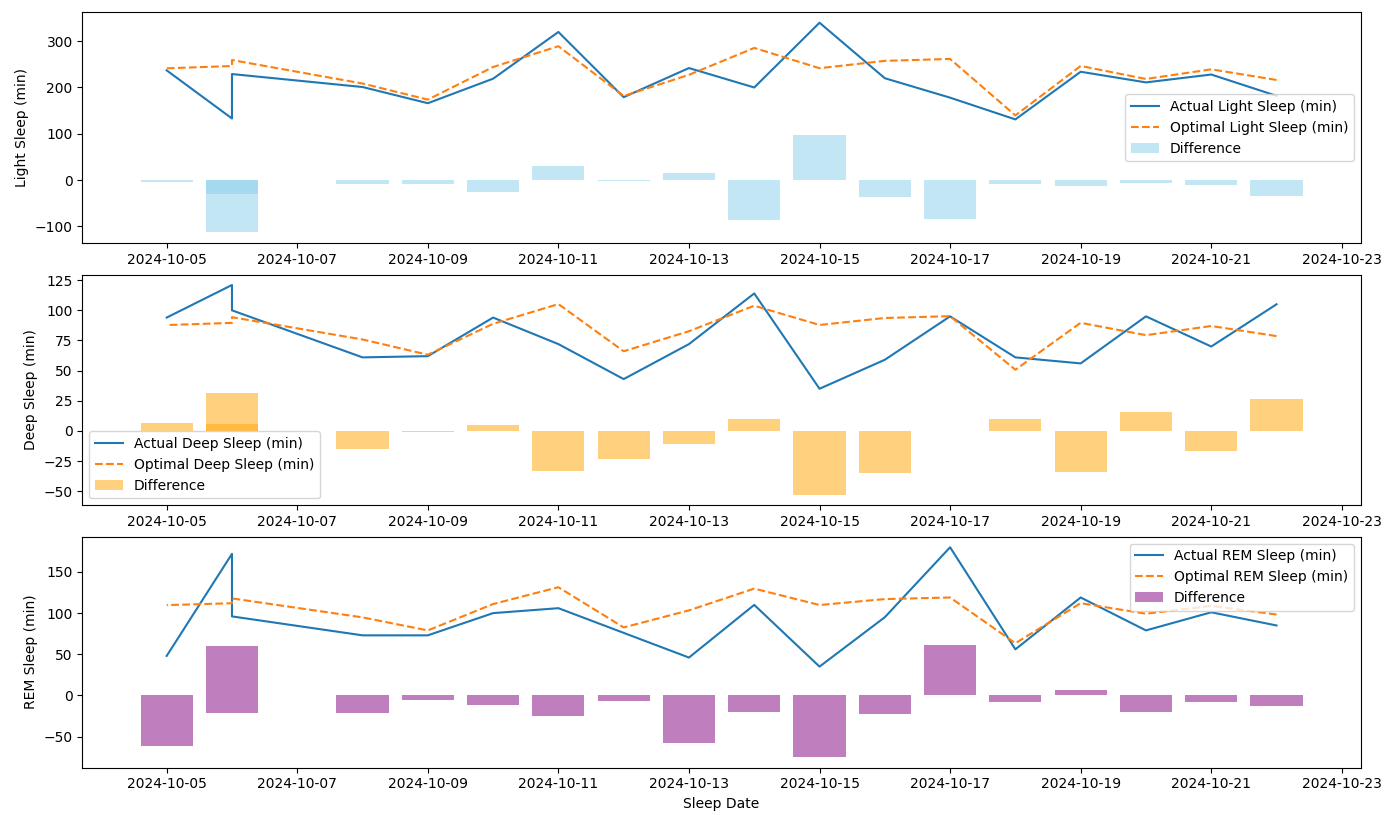
\includegraphics[width=0.8\textwidth]{SleepAnalysisByPhases.png}
        \caption{Sleep Performance Metrics as measured by the difference between optimal sleep and measured sleep.}
        \label{fig:sleep-metrics}
    \end{figure}
    \begin{figure}[H]
        \centering
        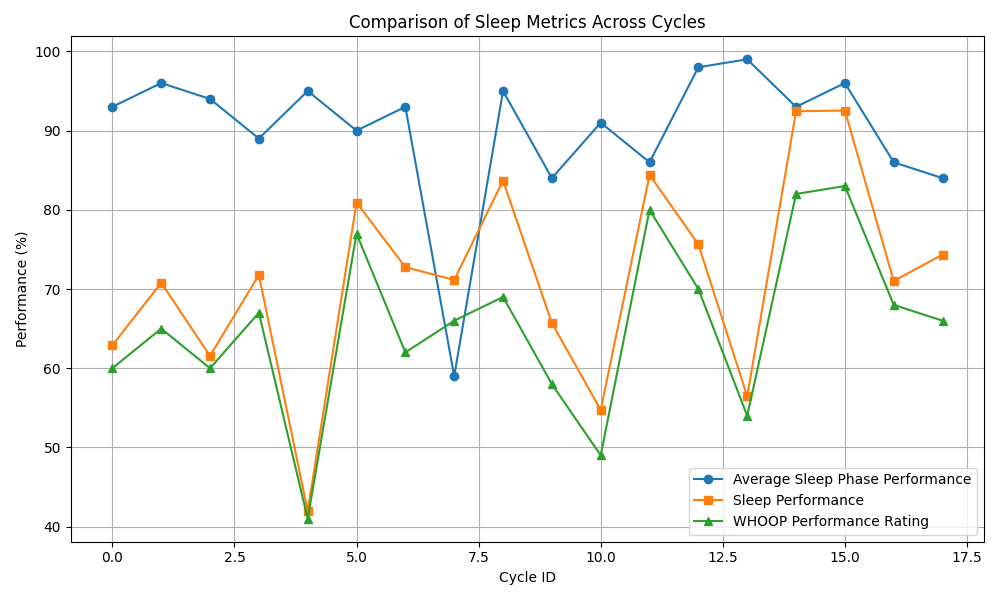
\includegraphics[width=0.8\textwidth]{SleepCycleComparison.png}
        \caption{Sleep Performance Metrics as measured by the difference between Whoop's performance rating and the average sleep performance and calculated sleep performance.}
        \label{fig:sleep-metrics}
    \end{figure}

\end{itemize}

\section{Future Work}
\begin{itemize}
    \item Final integration of graph and visualization components into the main system.
    \item Testing with simulated data to verify the accuracy of recommendations.
    \item Refinement of the user interface for seamless data interpretation.
\end{itemize}

\section{Appendix}
\subsection{Code Listings}
\begin{itemize}
    \item \texttt{SleepGraph.py}: The script that implements the graph-based system for analyzing sleep metrics.
    \item \texttt{sleepPlotRender.py}: The visualization script for generating plots of sleep performance metrics.
\end{itemize}

\end{document}
